\documentclass[12pt, titlepage]{article}

\usepackage{fullpage}
\usepackage[round]{natbib}
\usepackage{multirow}
\usepackage{booktabs}
\usepackage{tabularx}
\usepackage{graphicx}
\usepackage{float}
\usepackage{hyperref}
\hypersetup{
    colorlinks,
    citecolor=blue,
    filecolor=black,
    linkcolor=red,
    urlcolor=blue
}
\graphicspath{ {./images/} }

%% Comments

\usepackage{color}

\newif\ifcomments\commentstrue %displays comments
%\newif\ifcomments\commentsfalse %so that comments do not display

\ifcomments
\newcommand{\authornote}[3]{\textcolor{#1}{[#3 ---#2]}}
\newcommand{\todo}[1]{\textcolor{red}{[TODO: #1]}}
\else
\newcommand{\authornote}[3]{}
\newcommand{\todo}[1]{}
\fi

\newcommand{\wss}[1]{\authornote{blue}{SS}{#1}} 
\newcommand{\plt}[1]{\authornote{magenta}{TPLT}{#1}} %For explanation of the template
\newcommand{\an}[1]{\authornote{cyan}{Author}{#1}}

%% Common Parts

\newcommand{\progname}{ProgName} % PUT YOUR PROGRAM NAME HERE
\newcommand{\authname}{Team \#, Team Name
\\ Student 1 name and macid
\\ Student 2 name and macid
\\ Student 3 name and macid
\\ Student 4 name and macid} % AUTHOR NAMES                  

\usepackage{hyperref}
    \hypersetup{colorlinks=true, linkcolor=blue, citecolor=blue, filecolor=blue,
                urlcolor=blue, unicode=false}
    \urlstyle{same}
                                


\newcounter{acnum}
\newcommand{\actheacnum}{AC\theacnum}
\newcommand{\acref}[1]{AC\ref{#1}}

\newcounter{ucnum}
\newcommand{\uctheucnum}{UC\theucnum}
\newcommand{\uref}[1]{UC\ref{#1}}

\newcounter{mnum}
\newcommand{\mthemnum}{M\themnum}
\newcommand{\mref}[1]{M\ref{#1}}

\begin{document}

\title{System Design for \progname{}} 
\author{\authname}
\date{\today}

\maketitle

\pagenumbering{roman}

\section{Revision History}

\begin{tabularx}{\textwidth}{p{3cm}p{2cm}X}
\toprule {\bf Date} & {\bf Version} & {\bf Notes}\\
\midrule
Jan 18, 2023 & 1.0 & Revision 0\\
April 5, 2023 & 1.1 & Revision 1, UI updates\\
\bottomrule
\end{tabularx}

\newpage

\section{Reference Material}

This section records information for easy reference.

\subsection{Abbreviations and Acronyms}

\renewcommand{\arraystretch}{1.2}
\begin{tabular}{l l} 
    \toprule		
    \textbf{symbol} & \textbf{description}\\
    \midrule 
    AC & Anticipated Change\\
    DAG & Directed Acyclic Graph \\
    M & Module \\
    MG & Module Guide \\
    OS & Operating System \\
    R & Requirement\\
    SC & Scientific Computing \\
    SRS & Software Requirements Specification\\
    UC & Unlikely Change \\
    \bottomrule
  \end{tabular}\\

\newpage

\tableofcontents

\newpage

\listoftables

\listoffigures

\newpage

\pagenumbering{arabic}

\section{Introduction}

The following document details the System Design for \progname{}.\\
Relevant supporting documents include the System Requirement Specifications
and Module Guide. The full documentation and implementation can be
found at \url{https://github.com/mehtaj8/Greenway}.

\section{Purpose}

The purpose of this document is to outline the overall design of \progname{}. This document will cover what the user sees and interacts with, the software interface, descriptions and sketches of the user interaction experience along with a development timeline and reflection regarding the work on the system.\\

\noindent For more info, please refer to the other supporting documentation at \url{https://github.com/mehtaj8/Greenway}.

\section{Scope}
The scope of \progname{} requires the system to be able to integrate Google Maps API along with a car fuel economy database to determine and output a route optimized to minimize fuel costs. The system context can be visualized as follows: 
\begin{figure}[h!]
    \centering
    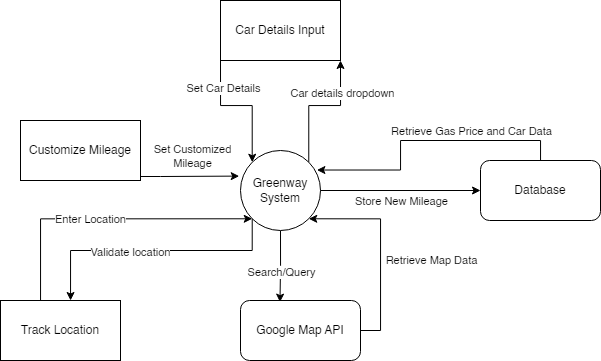
\includegraphics[scale=0.6]{Scope.png}
    \caption{System Context Diagram for Greenway}
\end{figure}

\section{Project Overview}

\subsection{Normal Behaviour}
Under normal circumstances, the system will have a general home screen that contains a display with text boxes to enter navigational start and end points, along with a menu to choose the car year, make, and model the trip will be completed in. The majority of the screen will include a map which will populate with the optimal route determined by the application. Once a route is determined. The system will also display the cheapest gas price in the area and calculate the cost of the trip using that information and the expected fuel consumption based on the car's fuel economy and elevation differences along the route.\\

\subsection{Undesired Event Handling}

The potential for a few undesired events and their handling procedures are outlined in the \href{https://github.com/mehtaj8/Greenway/blob/main/docs/HazardAnalysis/HazardAnalysis.pdf}{Hazard Analysis}.\\

\newpage
\subsection{Component Diagram}

\begin{figure}[h!]
    \centering
    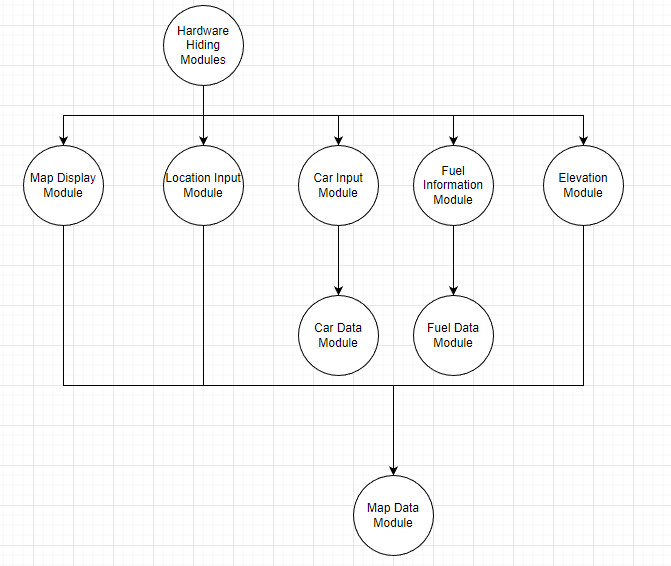
\includegraphics[scale=1]{images/component-diagram.png}
    \caption{Component Diagram}
\end{figure}

\subsection{Connection Between Requirements and Design} \label{SecConnection}

% \wss{The intention of this section is to document decisions that are made
%   ``between'' the requirements and the design.  To satisfy some requirements,
%   design decisions need to be made.  Rather than make these decisions implicit,
%   they are explicitly recorded here.  For instance, if a program has security
%   requirements, a specific design decision may be made to satisfy those
%   requirements with a password.}
The requirements were used to design the modules and similarly the UI. This can be seen in MG 
and MIS respectively with the traceability matrices found in the documents. 

\newpage

\section{User Interfaces}

\begin{figure}[h!]
    \centering
    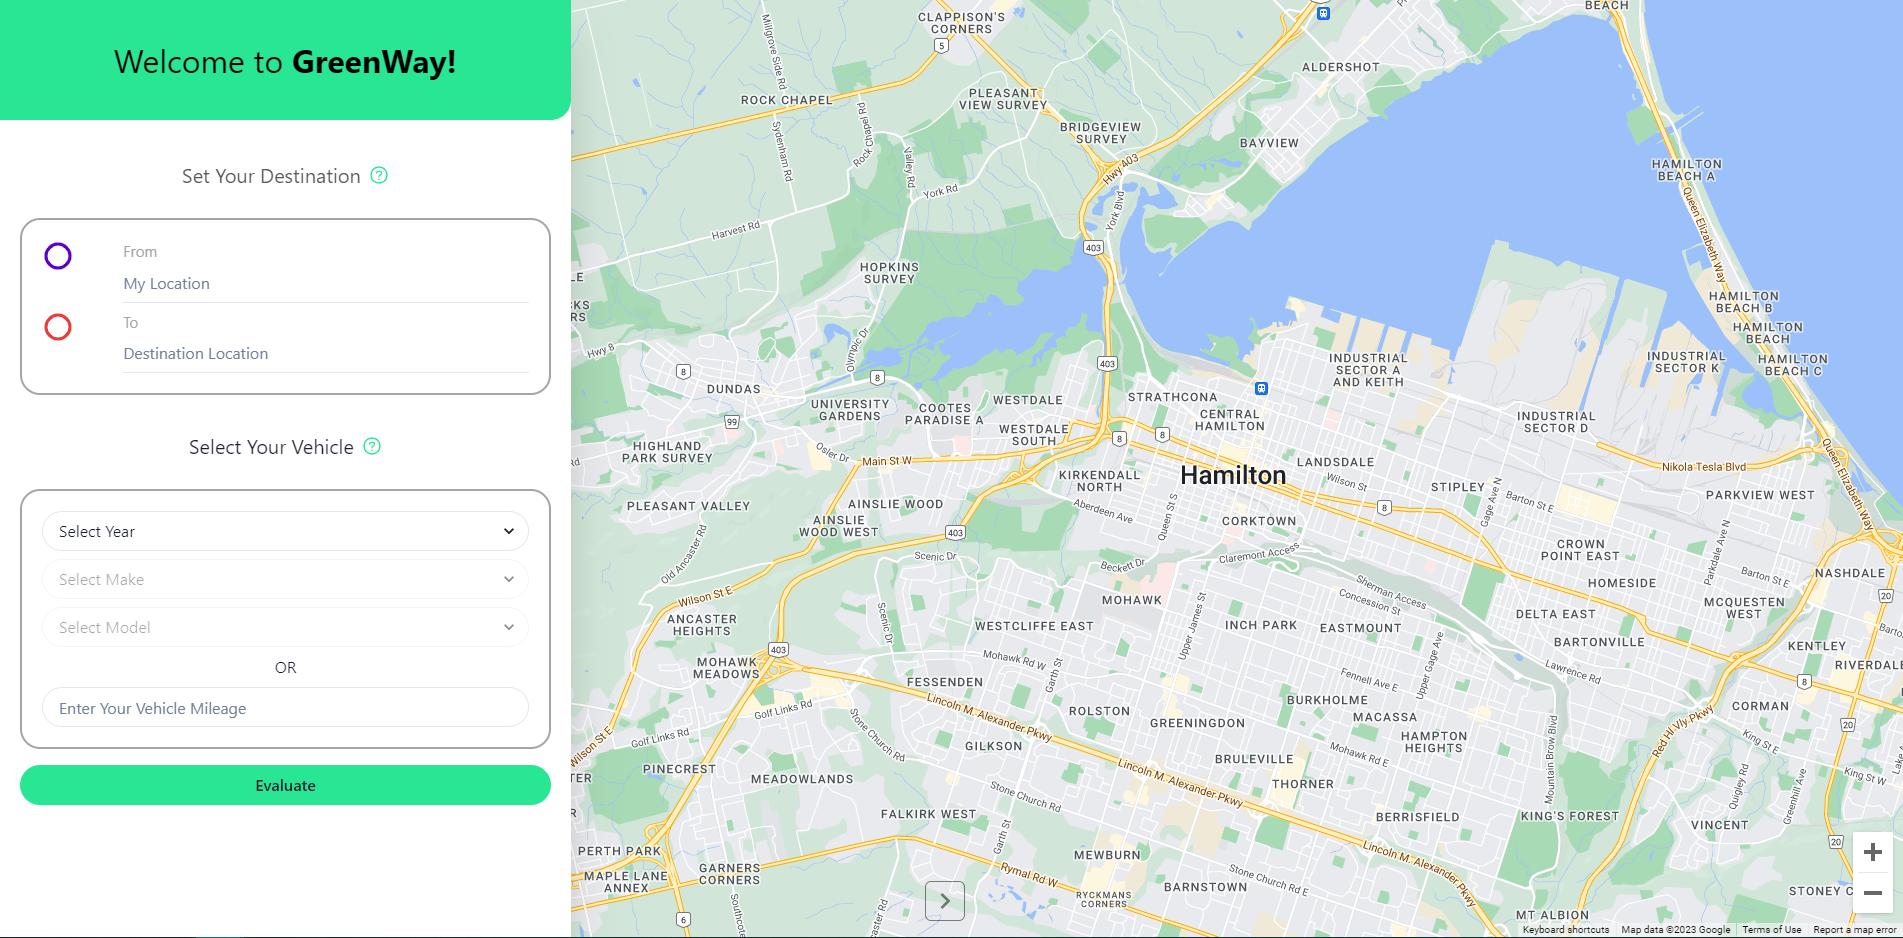
\includegraphics[scale=0.36]{landing-page.PNG}
    \caption{Landing Page}
\end{figure}
\begin{figure}[h!]
    \centering
    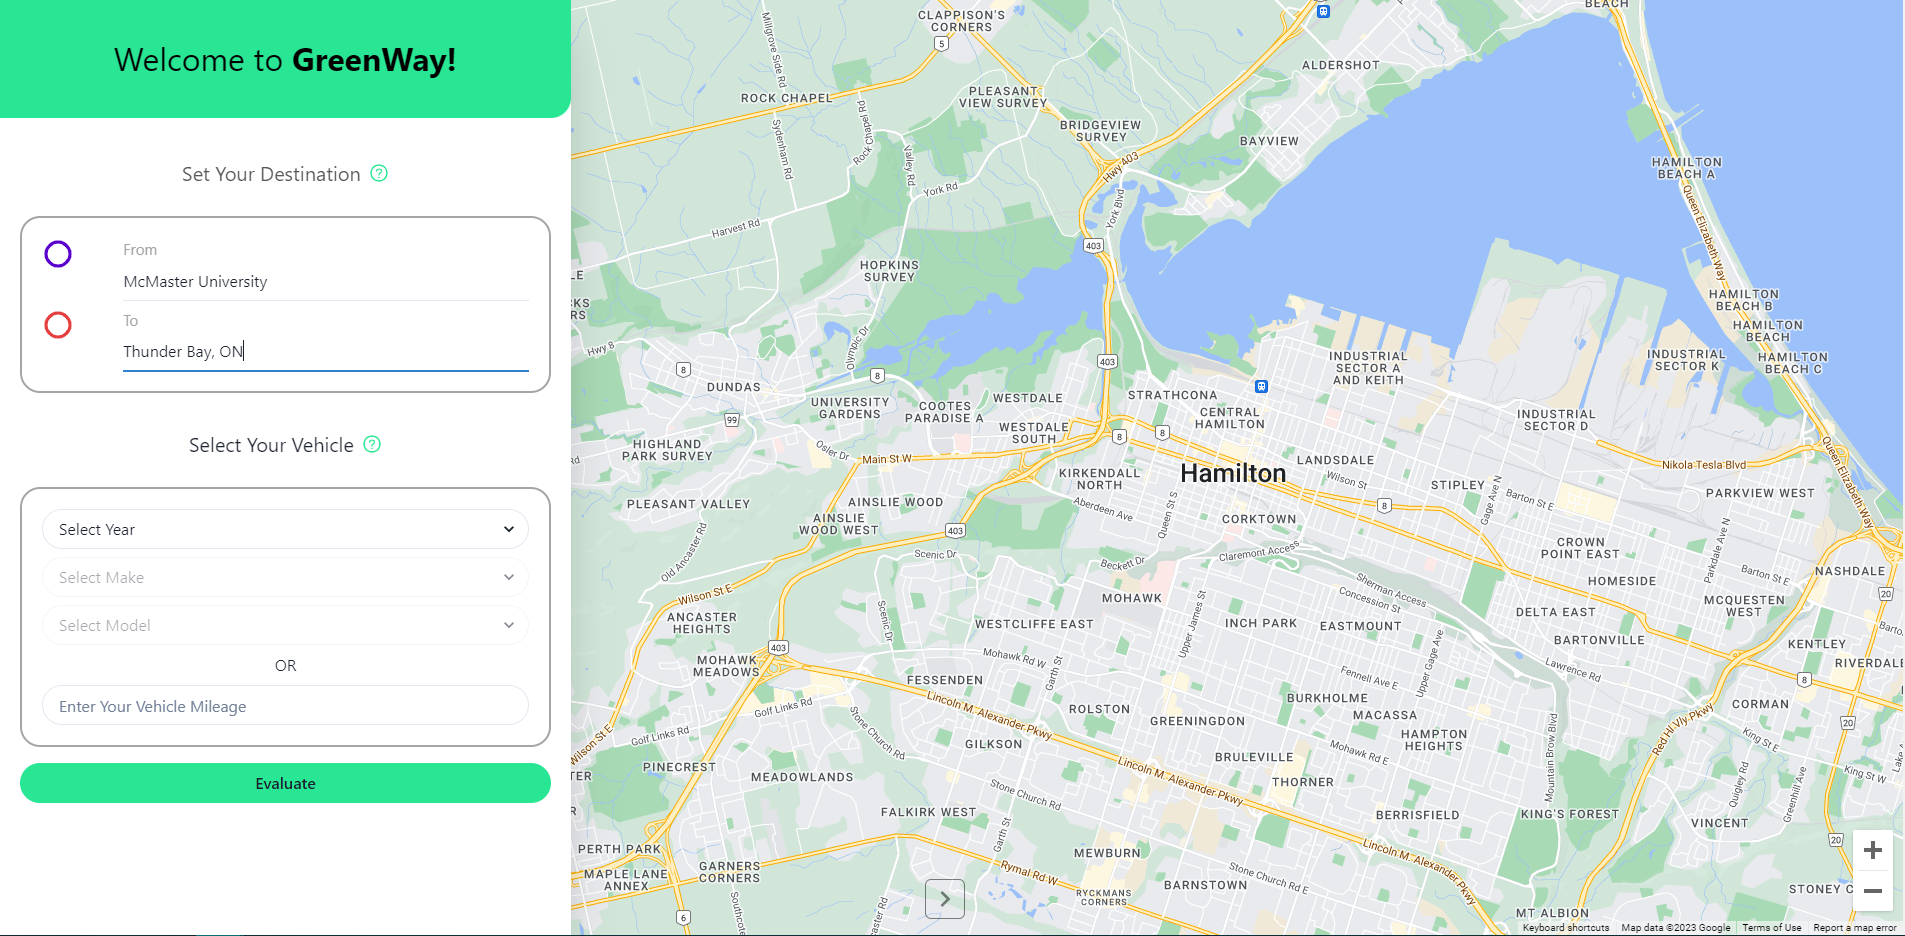
\includegraphics[scale=0.36]{location-selection.PNG}
    \caption{Location Selection}
\end{figure}
\begin{figure}[h!]
    \centering
    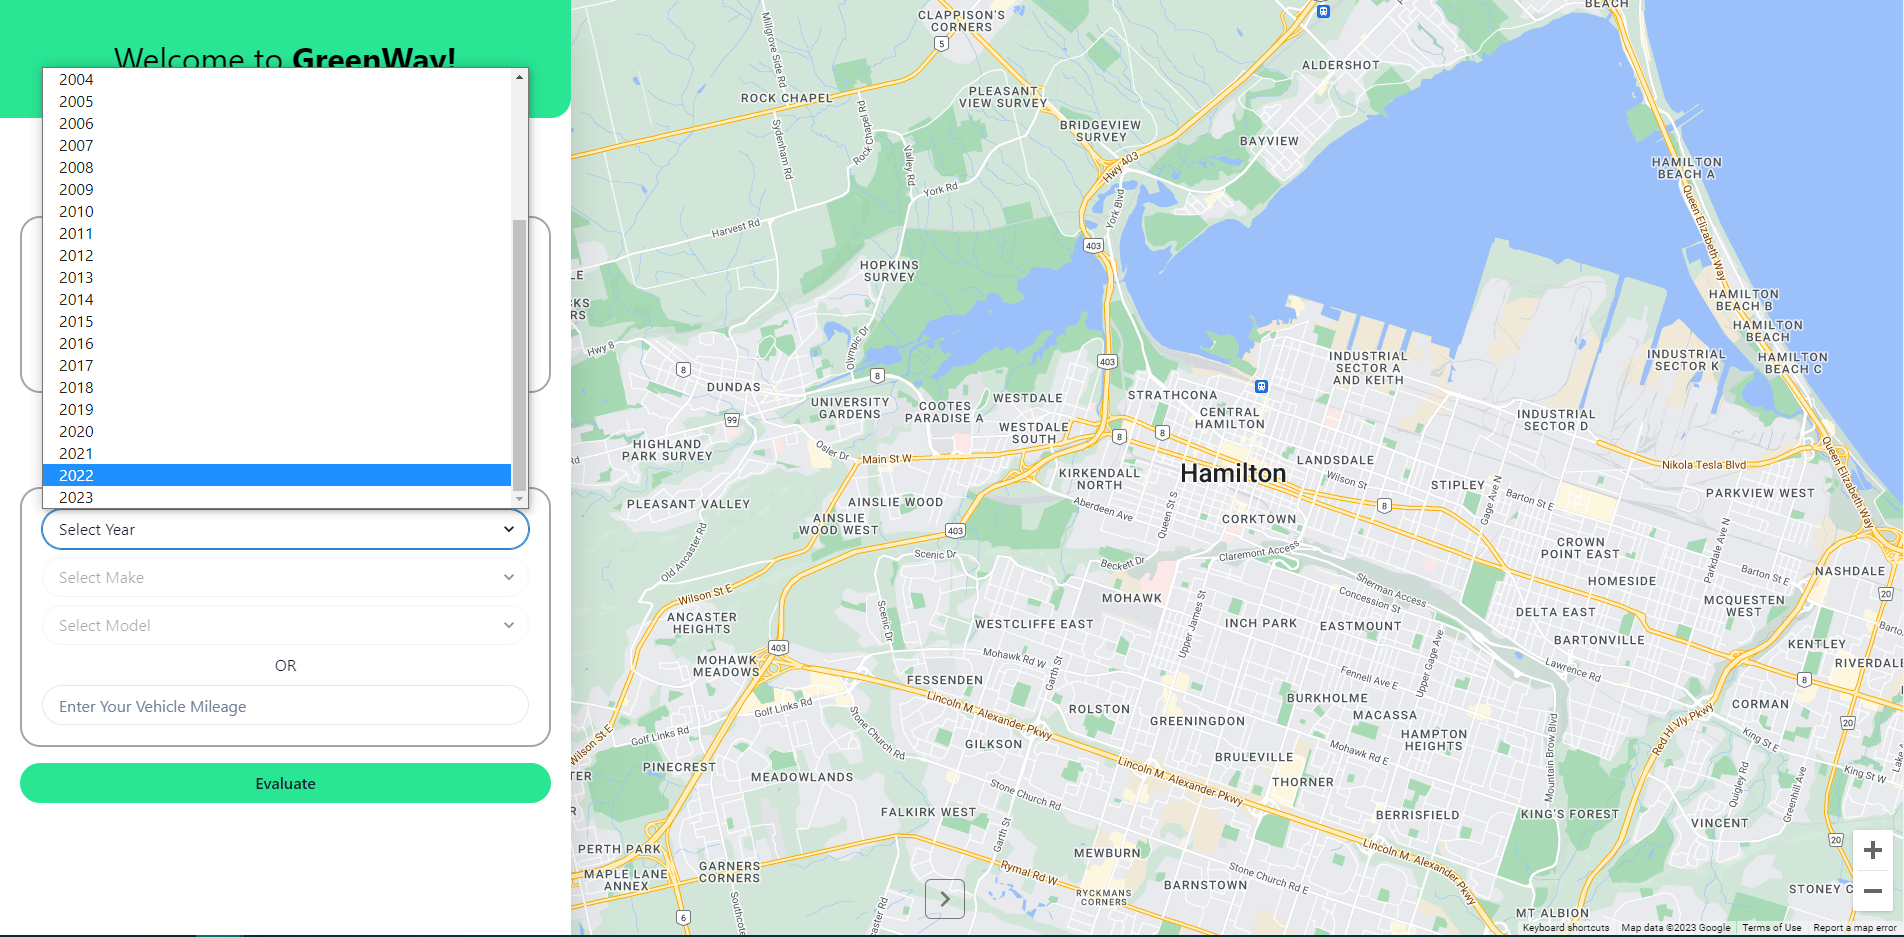
\includegraphics[scale=0.36]{select-year.PNG}
    \caption{Select Year}
\end{figure}
\begin{figure}[h!]
    \centering
    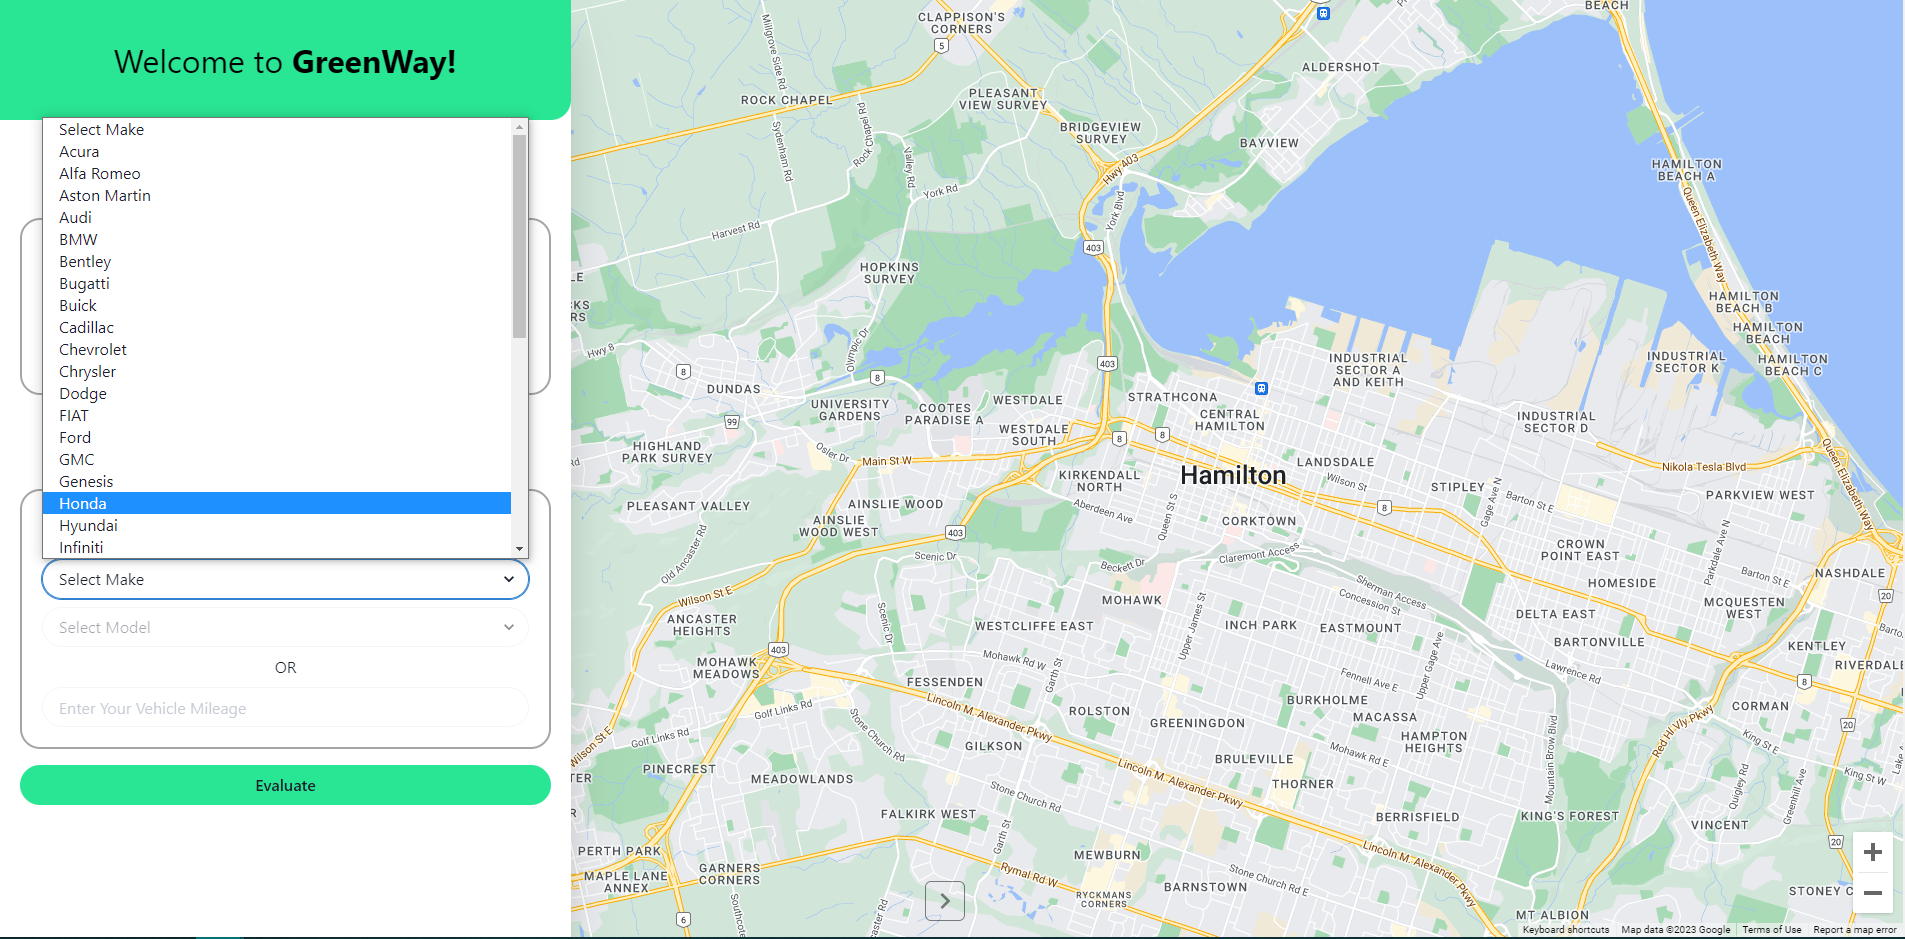
\includegraphics[scale=0.36]{select-make.PNG}
    \caption{Select Make}
\end{figure}
\begin{figure}[h!]
    \centering
    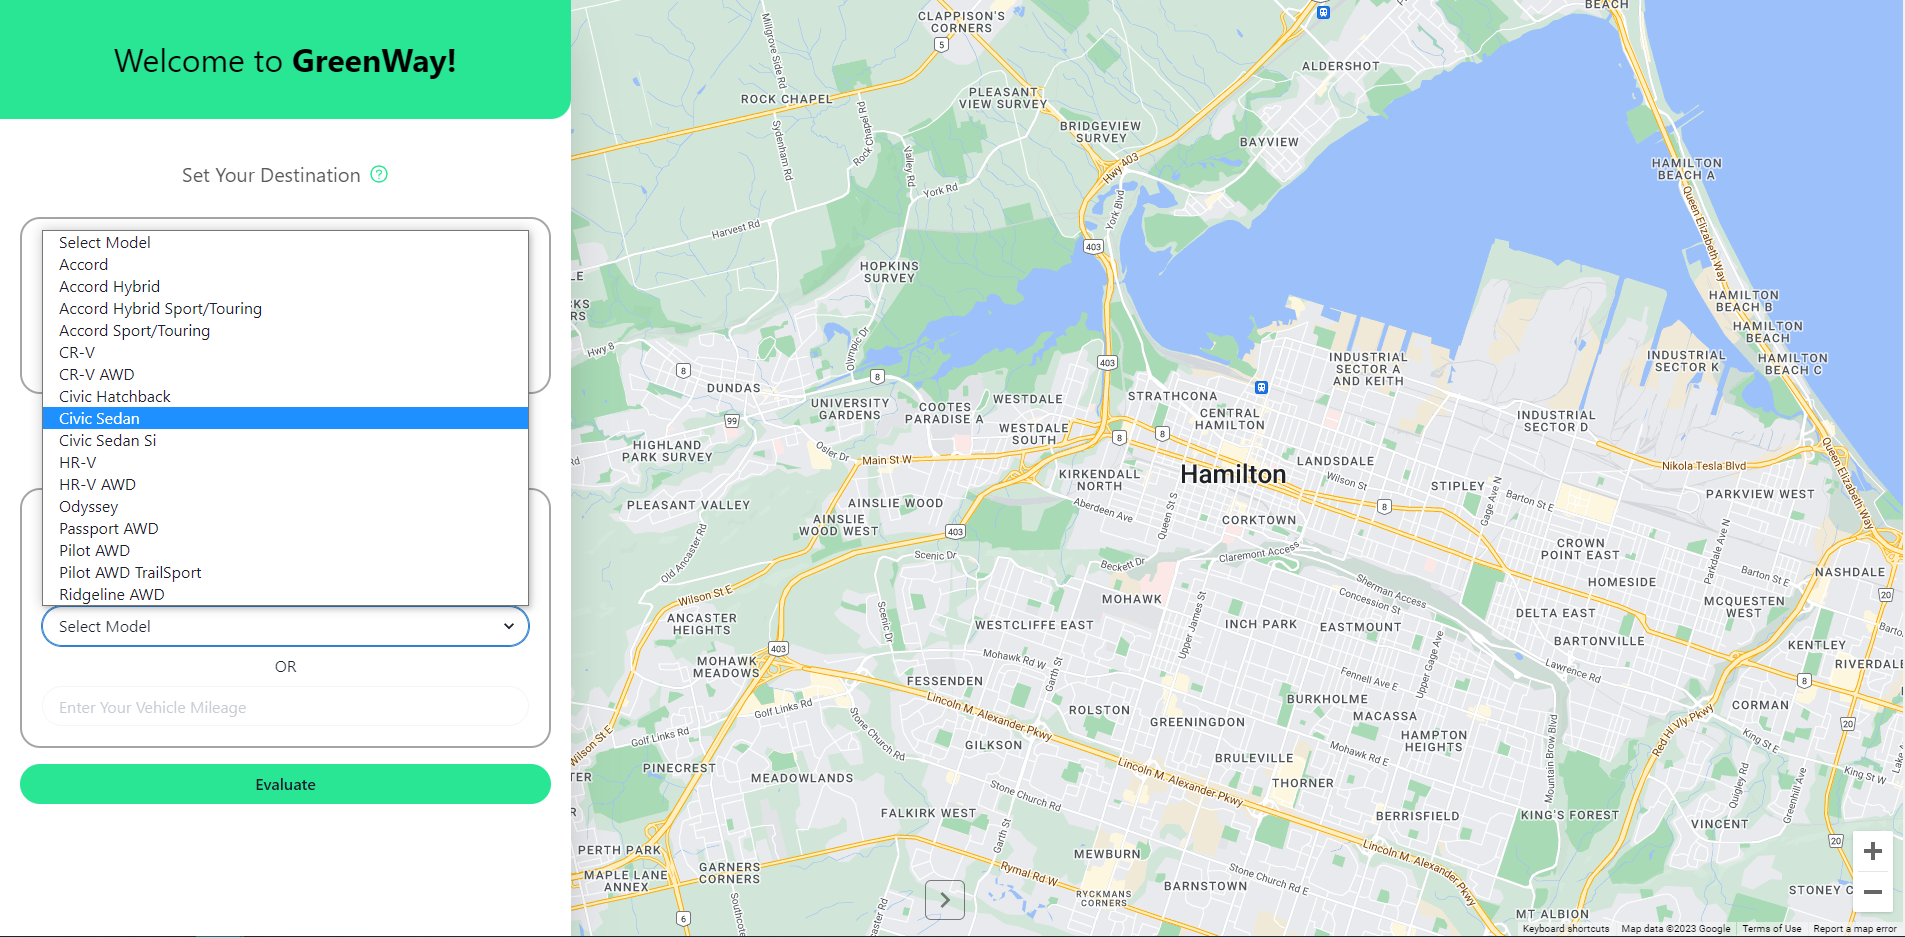
\includegraphics[scale=0.36]{select-model.PNG}
    \caption{Select Model}
\end{figure}
\begin{figure}[h!]
    \centering
    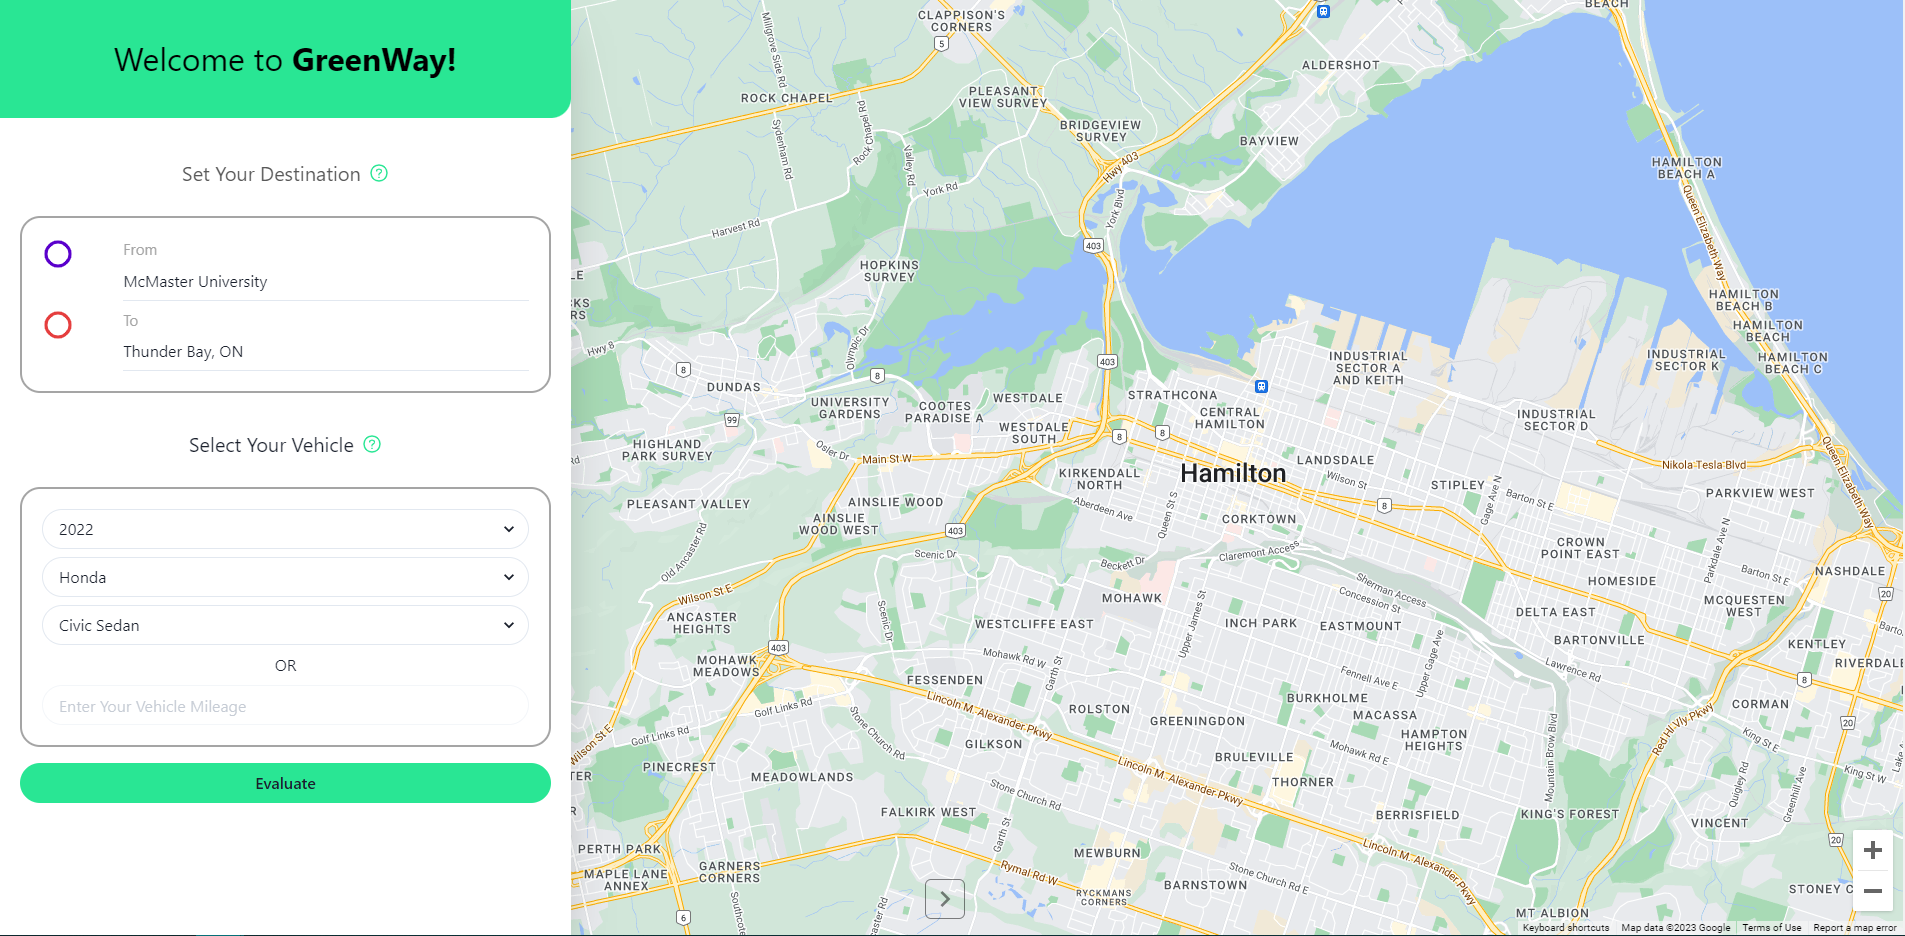
\includegraphics[scale=0.36]{correct-input.PNG}
    \caption{All inputs correct, Select Evaluate}
\end{figure}
\begin{figure}[h!]
    \centering
    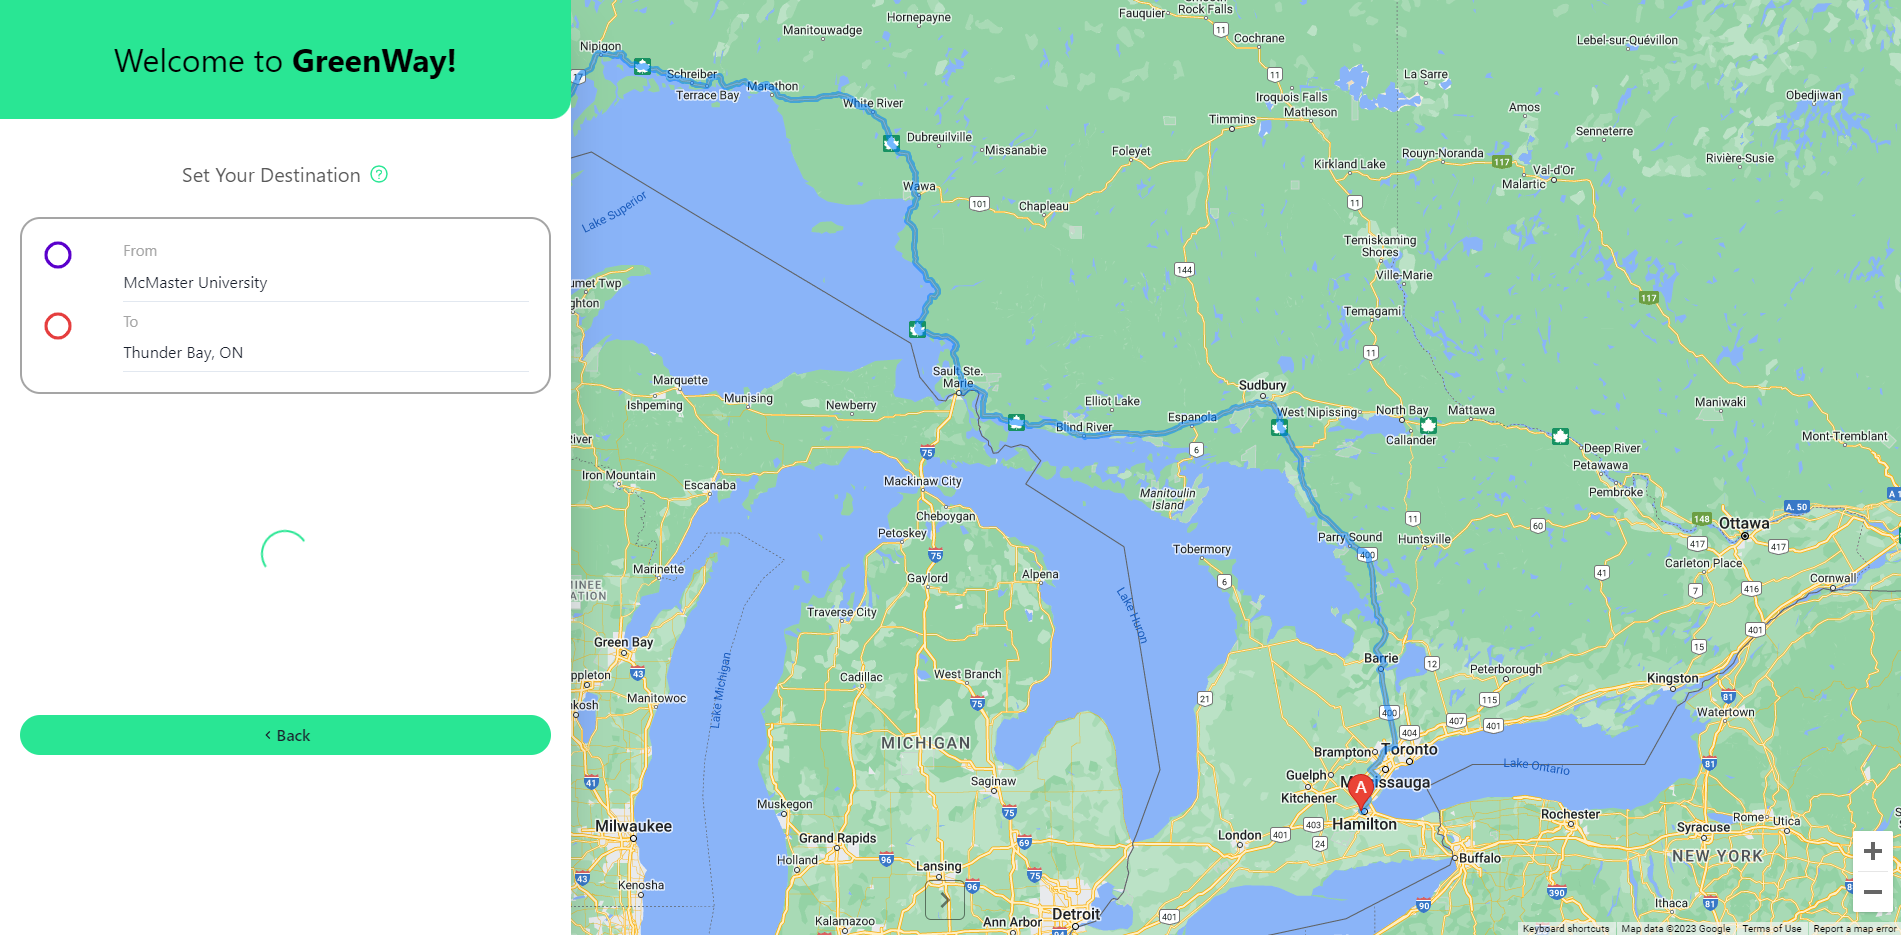
\includegraphics[scale=0.36]{loading.PNG}
    \caption{Loading, System performing calculations}
\end{figure}
\begin{figure}[h!]
    \centering
    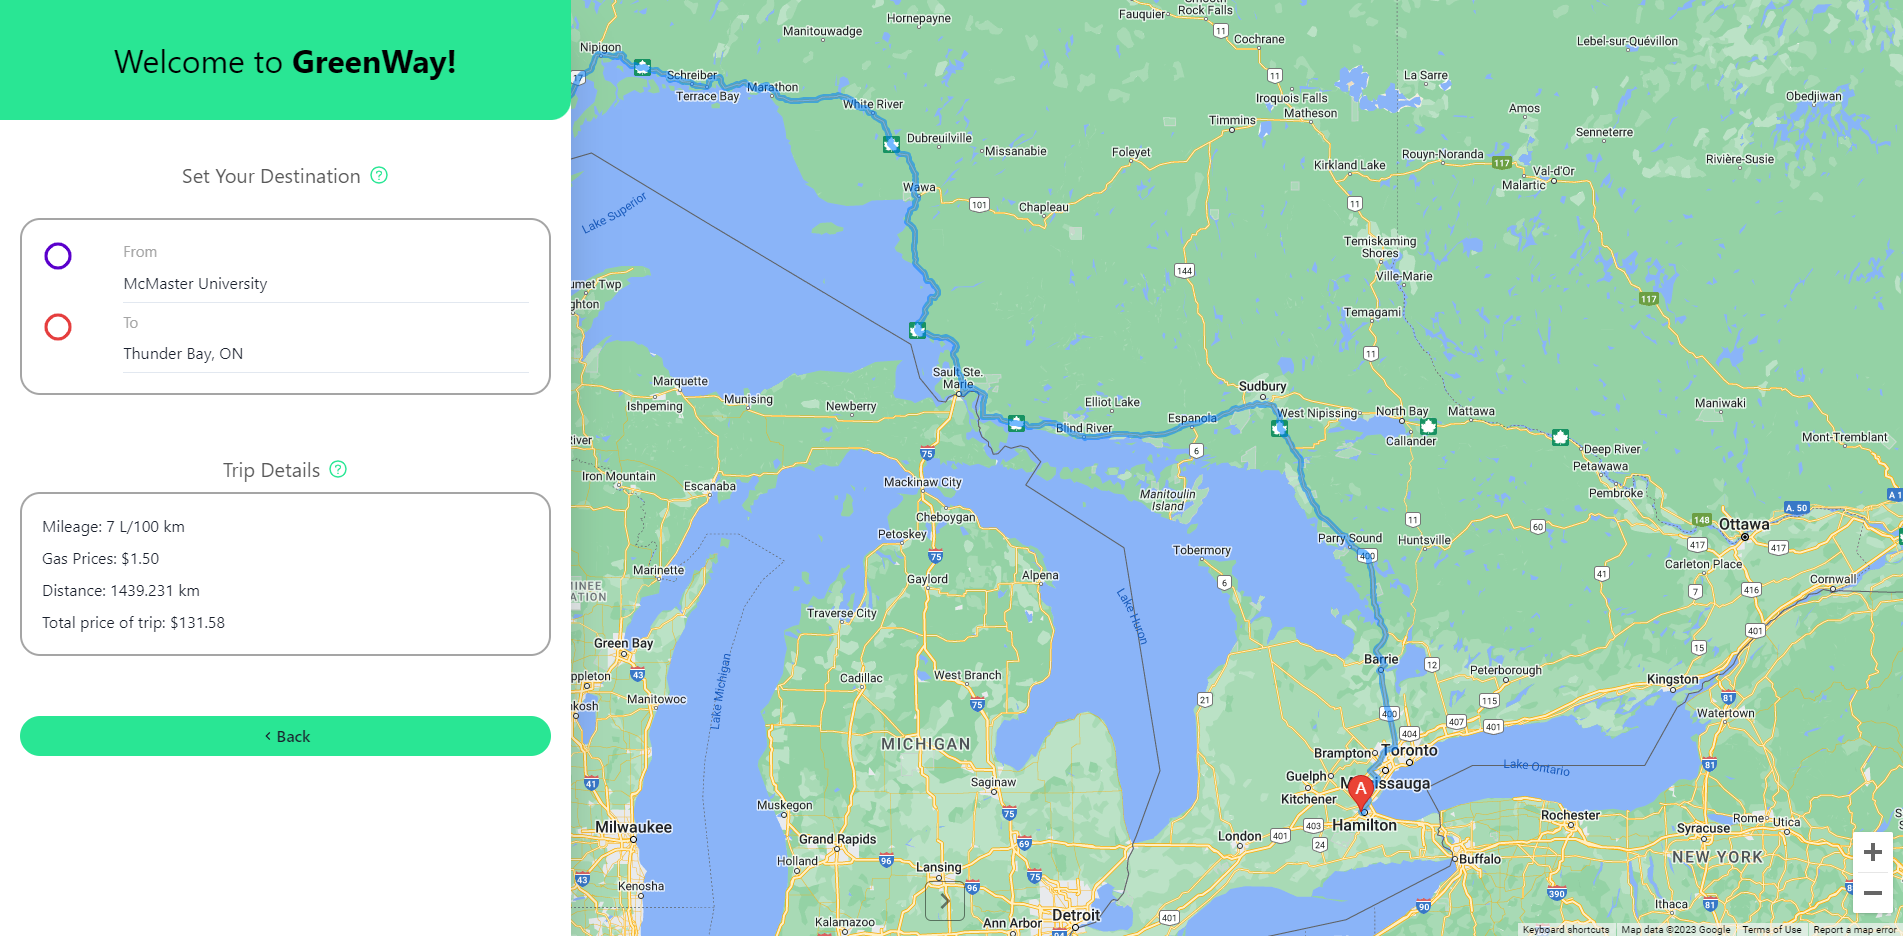
\includegraphics[scale=0.36]{total-cost.PNG}
    \caption{Total Price of Trip}
\end{figure}
\begin{figure}[h!]
    \centering
    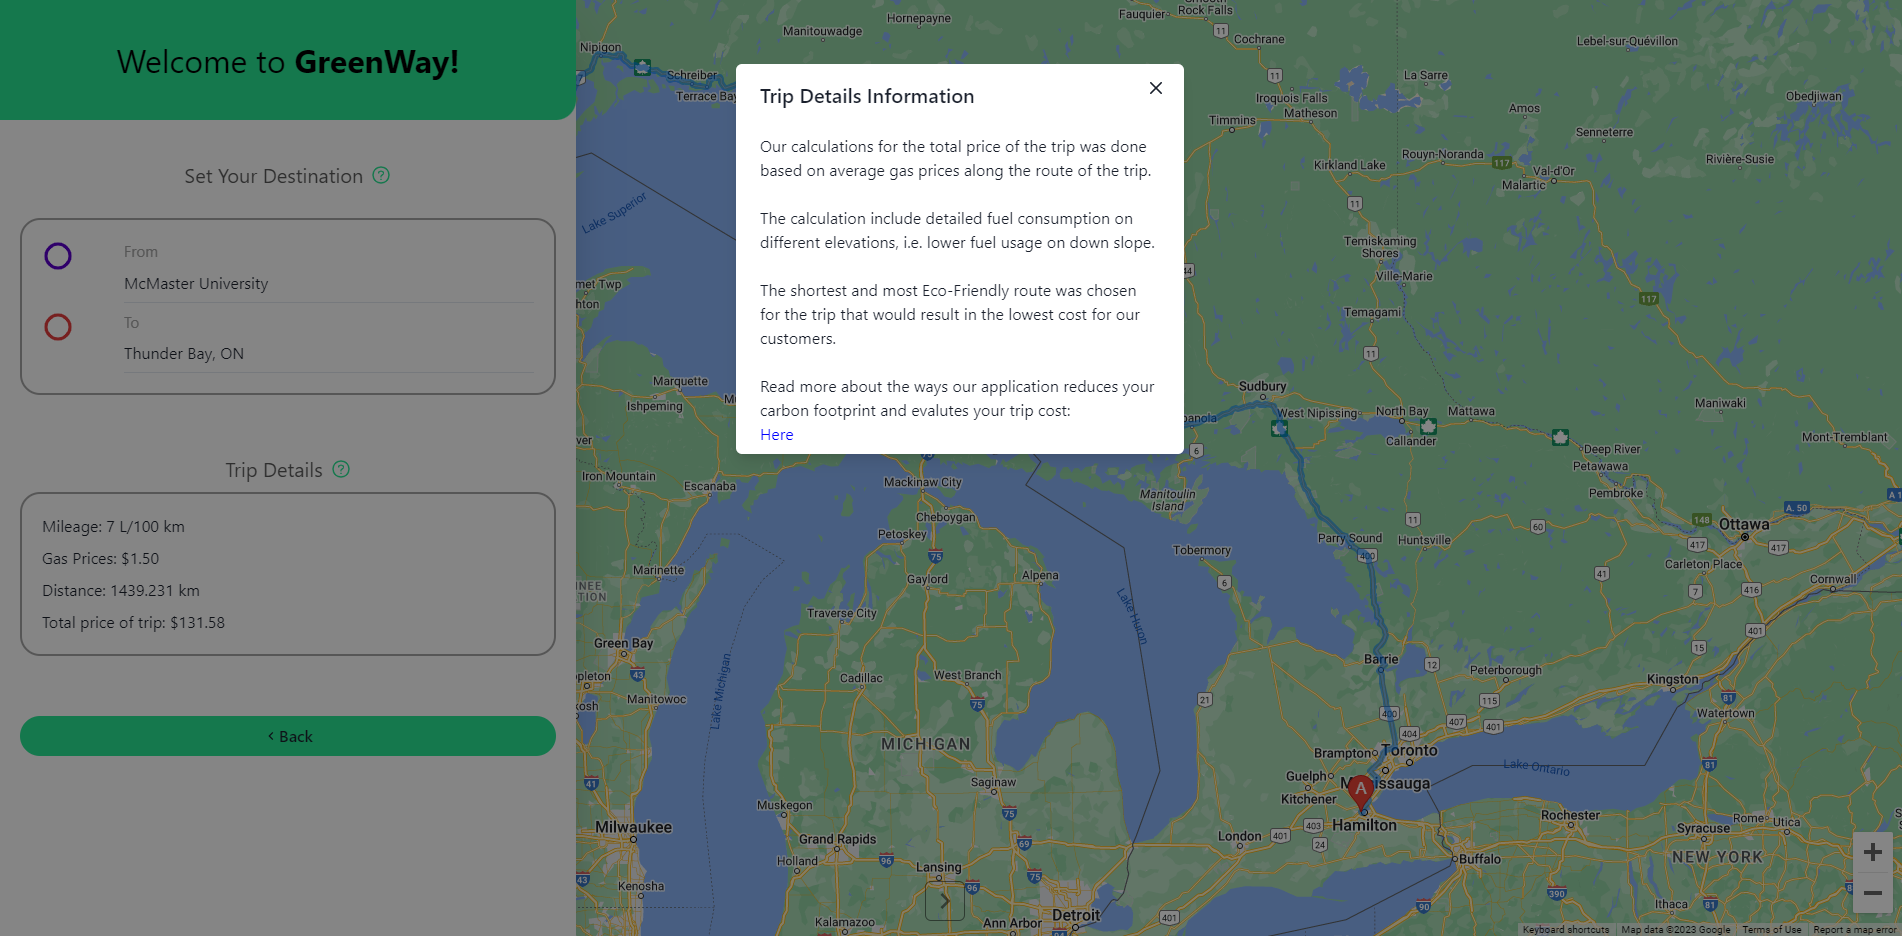
\includegraphics[scale=0.36]{trip-details.PNG}
    \caption{Trip Details}
\end{figure}

\newpage

\section{Design of Hardware}

No hardware is used in the system.

\section{Design of Electrical Components}

No electrical components are used in the system.

\section{Design of Communication Protocols}

No communication protocols are utilized in the system.

\section{Timeline}

\begin{table}[H]
	\begin{tabular}{|l|l|l|l|}
		\hline
		Component & Timeline Rev 0   & Timeline Final Rev & Who's Responsible \\ \hline
		Landing Page & February 13, 2023 & March 20, 2023     & Utsharga and Jash \\ \hline
		Location Selection & February 13, 2023 & March 20, 2023     & Utsharga and Priyansh \\ \hline
		Select Car Year, Make, Model & February 13, 2023 & March 20, 2023     & Utsharga and Priyansh \\ \hline
		Input Validation & February 13, 2023 & March 20, 2023     & Pranay and Jash \\ \hline
		Loading Screen & February 13, 2023 & March 20, 2023     & Bilal and Sharjil \\ \hline
		Total Cost Calculation & February 13, 2023 & March 20, 2023     & Bilal and Priyansh \\ \hline
		Trip Details & February 13, 2023 & March 20, 2023     & Bilal and Priyansh \\ \hline
	\end{tabular}
\end{table}

% \bibliographystyle {plainnat}
% \bibliography{../../../refs/References}

\newpage{}

\appendix

\section{Interface}

% \wss{Include additional information related to the appearance of, and
% interaction with, the user interface}
Figure (3-7): This is the start screen when launching the application. It allows the user to enter the start and end destination, along with there car details. The figures after figure 1 show the steps that can be taken by the user to enter there car details, and location details alike.\\
Figure (8): This screen show that the use can also enter there kust the mileage to replace car details.\\
Figure (9): This screen shows the result of the application along with the output that the app will give to the user with the total cost.\\
Figure (10): This screen shows extra information for the user to be able to understand the use of the application.\\

\section{Mechanical Hardware}
N/A

\section{Electrical Components}
N/A

\section{Communication Protocols}
N/A

\section{Reflection}

The information in this section will be used to evaluate the team members on the
graduate attribute of Problem Analysis and Design.  Please answer the following questions:

\begin{enumerate}
  \item What are the limitations of your solution?  Put another way, given
  unlimited resources, what could you do to make the project better? (LO\_ProbSolutions)\\ \\
  \textbf{Utsharga:} Our main features are reliant on the data provided by external APIs/ databases, especially the gas prices and car deatils. With unlimited resources, developing our own API with direct data from the sources would be ideal.\\
  \textbf{Jash:} Our application currently user specific accounts. With unlimited resources, creating the feature and providing user specific experience would be an amazing development.\\
  \textbf{Sharjil:} Our application currently does not use the hands-on domain, which limits the amount of testing needed to see how all the different parts of the project are integrated together to observe if the product is function as intended. \\
  \textbf{Bilal:} Our application doesn't have a well defined or correct way to find the impact of elevation on fuel consumption. This would be a topic of in depth research that could be used to make the cost estimations of this app more accurate.\\
  \textbf{Priyansh:} Our application does not provide navigation along the optimal route and only provides relevant fuel cost calculations. This is inconvenient in a real world scenario as most individuals rely on their phones to navigate, but they may not travel on the optimal route without noting down the suggested route by Greenway in advance.\\
  \textbf{Pranay:} Given unlimited resources and more advanced car technology, our application could theoretically connect to a car and receive direct and more accurate information regarding fuel efficiency and fuel consumption on paths with changes in elevation. Given unlimited resources, our app wouldn't have to be reliant on external APIs for data.\\
  
  \item Give a brief overview of other design solutions you considered.  What
  are the benefits and tradeoffs of those other designs compared with the chosen
  design?  From all the potential options, why did you select documented design? (LO\_Explores)\\ \\
  \textbf{Utsharga:} One of the other solutions included developing a mobile application instead of a web application. This had it's benefits as users are more likely to use an mobile application for travel purposes. However, this would also limit the number of users as the current team could only focus on one platform, i.e. iOS or Android. Our current application would translate to having mobile web view, enabling all users to be able to use it in all platforms.\\
  \textbf{Jash:} We considered parsing data live from different gas stations for accurate pricing with each usage of our application. This however would result in a lot of API calls and might result in slower performance of the application.\\
  \textbf{Sharjil:} Another solution that we considered was having the implementation of accounts system either internally within the website or through social media login instead of just using the website as a guest. The benefits would be that the routes that the people travelled on would be saved for their convenience. However, the storage of different users would cause a lot more strain on the back-end of the application, which is why we decided to not implement that idea. \\
  \textbf{Bilal:} One design solution we considered was using some common cars to represent the possible cars that the user can choose to represent there own car. This solution would reduce the load on our database to have a lot of cars available. But as a consequence would give a more inaccurate estimation for individuals who don't have that specific car.\\
  \textbf{Priyansh:} One of the other designs we considered involved using a more portable application available on Android or iOS that would provide navigation. One of the main benefits to this over the one we settled on would be the ability to follow the suggested route, however a key drawback was that many other apps currently offer navigation, and it would distract from the core purpose of the application which is to determine and minimize fuel costs on a given trip.\\
  \textbf{Pranay:} There were various design options we had to choose between while developing our project Greenway. One of the design decisions we had to make was whether to create a web application or a mobile application. The advantages of sticking with a web application were greater accessibility and our team was more familiar with web development. Creating a mobile application might have forced us to choose either Android or Apple. It was unrealistic to attempt to create the application on both platforms given time constraints.\\
\end{enumerate}

\end{document}